% !TeX root = ./pf.tex

%\includeonlyframes{current}

\section*{Abstraction}

\begin{frame}{Abstraction}

  \centering\large\textit{The process of \textbf{highlighting} important
    aspects\\and \textbf{hiding} unimportant details about an idea}

  \vfill

  \begin{itemize}
  \item<2-> Essential to build \textbf{reusable} software components and
    meaningful software products
  \item<3-> For code: basic instructions $\to$ functions $\to$ invocables
  \item<4-> For data: fundamental types $\to$ data structures $\to$ templates
  \end{itemize}
\end{frame}

\section*{Code abstraction -- Functions}

\begin{frame}[fragile]{Functions}

  \begin{itemize}[<+->]
  \item A function abstracts a piece of code that performs a well-defined task
    behind a well-defined interface
  \item A function associates a block of statements with
    \begin{itemize}
    \item a name
    \item a list of zero or more parameters
    \end{itemize}
  \item A function may return a result
  \end{itemize}

  \begin{itemize}[<+->]
  \item Let's consider the code that computes the integer square root
    \begin{itemize}
    \item Let's give it a name $\rightarrow$ \code{isqrt}
    \item We pass \code{isqrt} a number $\rightarrow$ the list of parameters has
      only one item of type \code{int}
    \item \code{isqrt} computes a value that we want back $\rightarrow$ the
      function returns a value of type \code{int}
    \end{itemize}
  \end{itemize}

  \begin{itemize}[<+->]
  \item \href{https://isocpp.github.io/CppCoreGuidelines/CppCoreGuidelines#f1-package-meaningful-operations-as-carefully-named-functions}{F.1}, \href{https://isocpp.github.io/CppCoreGuidelines/CppCoreGuidelines#f10-if-an-operation-can-be-reused-give-it-a-name}{F.10}
  \end{itemize}
\end{frame}

\begin{frame}[fragile]{The \code{isqrt} function}

  \begin{columns}[T]
    \begin{column}{.4\textwidth}
      \begin{codeblock}
#include <iostream>

int main()
\{
  int n;
  std::cin >{}> n;
  int i\{1\};
  while (i * i < n) \{
    ++i;
  \}
  if (i * i > n) \{
    --i;
  \}
  std::cout << i << \bslashn;
\}\end{codeblock}

      \vskip .5cm

      \uncover<2>{Names on the two sides of the call are independent}
    \end{column}

    \begin{column}{.6\textwidth}
      \begin{codeblock}
#include <iostream>

int isqrt(int \alert<2>{n})  \only<1>{// \alert{function definition}}
\{
  int i\{1\};
  while (i * i < n) \{
    ++i;
  \}
  if (i * i > n) \{
    --i;
  \}
  return \alert<2>{i};      \only<1>{// \alert{return statement}}
\}

int main()
\{
  int \alt<1>{n}{\alert<2>{num}};
  std::cin >{}> \alt<1>{n}{\alert<2>{num}};
  int \alt<1>{i}{\alert<2>{result}}\{isqrt(\alt<1>{n}{\alert<2>{num}})\};  \only<1>{// \alert{function call}}
  std::cout <{}< \alt<1>{i}{\alert<2>{result}} <{}< \bslashn;
\}\end{codeblock}
    \end{column}

  \end{columns}

\end{frame}

\begin{frame}[fragile]{Function declaration}

  \begin{itemize}[<+->]
  \item A function \alert{declaration} contains the essential information needed
    to call (or invoke) the function

    \textit{return-type} \textit{function-name} \code{(} \textit{parameter-list} \code{);}

  \item If the declaration is followed by the actual block of statements (the
    \textit{implementation} of the function), it is also a \alert{definition}

    \textit{return-type} \textit{function-name} \code{(} \textit{parameter-list} \code{) \{ \ddd{} \}}

    \begin{itemize}
    \item Note the block scope
    \end{itemize}

  \item Each parameter in the parameter list is of the form

    \textit{type \opt{name}}

    \begin{itemize}
    \item \textit{type} is mandatory
    \item \textit{name} is optional
      \begin{itemize}
      \item in the declaration, but useful for documentation purposes
      \item in the definition if it's not used
        (\href{https://isocpp.github.io/CppCoreGuidelines/CppCoreGuidelines#f9-unused-parameters-should-be-unnamed}{F.9})
      \end{itemize}

    \end{itemize}
    

  \end{itemize}
\end{frame}

\begin{frame}[fragile]{Function declaration \insertcontinuationtext}

  \begin{itemize}[<+->]
  \item Parameters are separated by commas

  \item The parameter list can be empty, i.e. \code{()}

  \item If the function returns nothing, the return type is \code{void}

  \end{itemize}

  \begin{codeblock}<+->{
int isqrt(int);                        // declaration
int count_words(std::string s) \{ \ddd \}  // definition
double pow(double base, double exp);   // declaration
void print(std::string);               // declaration
int generate_random_number() \{ \ddd \}    // definition}\end{codeblock}

\end{frame}

\begin{frame}[fragile]{Returning from a function}

  \begin{itemize}[<+->]
  \item Within the function block, the \alert{\code{return}} statement returns
    the result (and the control) to the calling function

  \item For a function returning a non-\code{void} type

    \code{return} \textit{expression} \code{;}

    The result of \textit{expression} must be convertible to the return type

  \item For a function returning \code{void}

    \code{return;}

    At the end of the function, \code{return;} is optional

  \end{itemize}

\end{frame}

\begin{frame}[fragile]{Returning from a function \insertcontinuationtext}

  \begin{itemize}
  \item A function has only one entry point, but it may have multiple exit
    points, i.e. there can be multiple \code{return} statements

    \begin{codeblock}
bool is_prime(int n) \{
  // simple cases
  if (n == 2) \{ \alert{return} true; \}
  if (n == 1 || n \% 2 == 0) \{ \alert{return} false; \}

  // complex cases
  \ddd

  \alert{return} result;
\}\end{codeblock}

    \end{itemize}

\end{frame}

\begin{frame}[fragile]{Invoking a function}

  \begin{itemize}
  \item Invoking/calling a function is a type of expression of the form $F(E_1,
    E_2, \ldots, E_N)$
    \begin{itemize}
    \item $F$ is an expression that identifies a function, typically its name
    \item The $E_i$'s are expressions, whose values are ``passed'' to the function
    \end{itemize}

    \begin{codeblock}<2->{
int s = isqrt(24);
std::cout <{}< count_words("Hello, " + name);
print(std::to_string(pow(isqrt(24), 2)));}\end{codeblock}

  \item<3-> Given a function

  % \tikzref doesn't work inside \code nor inside \texttt; to be investigated

    \begin{equation*}
      \code{R F(T$_1$ p}\tikzref{p1}\code{$_1$, \ddd, T$_n$ p}\tikzref{pn}\code{$_n$) \{ \ddd{} return E}\tikzref{er}\code{$_R$; \} }
    \end{equation*}

    and a function call

    \begin{equation*}
      \code{R r}\tikzref{r}\code{ = F(E}\tikzref{e1}\code{$_1$, \ddd, E}\tikzref{en}\code{$_n$);}
    \end{equation*}

    \begin{itemize}
    \item<4-> Each \code{p$_i$} is initialized with the value of expression
      \code{E$_i$}
    \item<5-> \code{r} is initialized with the value of expression \code{E$_R$}
    \end{itemize}

    \visible<4->{
      \tikz[remember picture, overlay] \draw[-Stealth,blue,line width=1pt] ([yshift=1ex] e1) -- ([yshift=-1ex]p1);
      \tikz[remember picture, overlay] \draw[-Stealth,blue,line width=1pt] ([yshift=1ex] en) -- ([yshift=-1ex]pn);
    }
    \visible<5->{
      \tikz[remember picture, overlay] \draw[-Stealth,brown,line width=1pt] ([yshift=-1ex] er) -- ([yshift=1ex]r);
    }

  \end{itemize}

\end{frame}

\begin{frame}[fragile]{Invoking a function \insertcontinuationtext}

  \begin{itemize}
  \item A function needs to be declared before it’s used
  \item The definition can appear later

    \begin{columns}[T]<.->
      \begin{column}<.->{.33\textwidth}
        \begin{codeblock}<.->{
int main()
\{
  \ddd
  isqrt(num); // error
  \ddd
\}

int isqrt(int n)
\{
   \ddd
\}}\end{codeblock}
      \end{column}
      \begin{column}{.33\textwidth}<.->
        \begin{codeblock}<.->{
int isqrt(int n)
\{
  \ddd
\}

int main()
\{
  \ddd
  isqrt(num); // ok
  \ddd
\}}\end{codeblock}
      \end{column}
      \begin{column}{.33\textwidth}<.->
        \begin{codeblock}<.->{
int isqrt(int);

int main()
\{
  \ddd
  isqrt(num); // ok
  \ddd
\}

int isqrt(int n)
\{
  \ddd
\}}\end{codeblock}
      \end{column}
    \end{columns}

  \end{itemize}

\end{frame}

\begin{frame}[fragile]{Function definition}

  \begin{itemize}[<+->]

  \item The lifetime of parameters ends at the end of the block
    
    \begin{codeblock}<.->{
bool is_prime(int n)
\{
  \ddd n \ddd
\} // the lifetime of n ends here}\end{codeblock}

  \item A function can call other functions

    \begin{codeblock}<.->{
bool is_prime(int n)
\{
  \ddd
  int div\{2\};
  int const s\{\alert{isqrt}(n)\};
  while (div <= s) \{
  \ddd
\}}\end{codeblock}

  \item A function should not be too long
    (\href{https://isocpp.github.io/CppCoreGuidelines/CppCoreGuidelines#f3-keep-functions-short-and-simple}{F.3})

  \item A function should perform a single logical operation
    (\href{https://isocpp.github.io/CppCoreGuidelines/CppCoreGuidelines#f2-a-function-should-perform-a-single-logical-operation}{F.2})

  \item Split long/complex functions into multiple parts, each implemented as a
    function
  \end{itemize}

\end{frame}

\begin{frame}[fragile]{How do we know the code we write is correct?}

  \begin{itemize}[<+->]
  \item Correctness is the absence of defects (also known as bugs) in a software
  \item Correctness is the result of the application of multiple good practices
    to the software developmente process
  \item One of the most effective techniques is \textbf{testing}
    \begin{itemize}
    \item Execute the code with reasonable and unreasonable input and see if it
      behaves according to the expectations
    \item The purpose of testing is to (try to) \alert{break} the code
    \end{itemize}
  \end{itemize}

  \uncover<+->{\centering\textbf{\alert{Testing can reveal the presence of bugs,\\not prove their
      absence!}}}

  \begin{itemize}[<+->]
  \item Here we focus on a form of testing called \textit{unit testing}, where
    the units (of code) under test are, for example, functions
  \item There are many tools/frameworks to do unit testing (Google Test, Catch,
    Doctest, Boost.Test, \ldots)
  \item Let's use Doctest (\url{https://github.com/doctest/doctest})
  \end{itemize}

\end{frame}

\begin{frame}[fragile]{How to use Doctest}

  \begin{itemize}
  \item On \href{https://godbolt.org/}{Compiler Explorer} it's available
    selecting it under ``Libraries''
  \item Otherwise download locally a single
    \href{https://raw.githubusercontent.com/doctest/doctest/master/doctest/doctest.h}{\textit{header
        file}} into the directory containing your code, e.g. using \code{wget}
    or \code{curl}
  \item At the top of your \Cpp{} file add the lines
    \begin{codeblock}
#define DOCTEST\_CONFIG\_IMPLEMENT\_WITH\_MAIN
#include "doctest.h"\end{codeblock}
  \item Don't add \code{main} into your file
  \item After the declarations of the function(s) you want to test, add lines
    like the following:
    \begin{codeblock}
TEST_CASE("Testing isqrt") \{
  CHECK(isqrt(0) == 0);
  CHECK(isqrt(9) == 3);
  CHECK(isqrt(10) == 3);
  CHECK(isqrt(-1) == 0);
  \ddd
\}\end{codeblock}

  \end{itemize}

\end{frame}

\begin{frame}[fragile]{The \code{main} function}
  \begin{itemize}
  \item The \code{main} (special) function is the entry point of a program
  \item It can have two forms
    \begin{itemize}
    \item \code{int main() \{\ddd\}}
    \item \ldots (see later)
    \end{itemize}
  \item<2-> If there is no \code{return} statement at the end, an implicit\\
    \code{return 0;} is assumed
    \begin{itemize}
    \item $0$ means success, different from $0$ means failure
    \item Or use \code{EXIT_SUCCESS} and \code{EXIT_FAILURE} from \code{<cstdlib>}
    \item The returned value is available to the shell via the \code{\$?}
      variable
    \end{itemize}
  \end{itemize}

  \begin{codeblock}<2->{
#include <cstdlib>

int main() \{
  int n;
  std::cin >> n;
  if (std::cin.fail() || n < 0) \{
    std::cerr << "Invalid number\bslash{}n";
    return EXIT_FAILURE;
  \}
  \ddd
\}}\end{codeblock}

\end{frame}

\begin{frame}[fragile]{Recursive functions}

  \begin{itemize}
  \item A function can call itself, directly or indirectly
    \begin{itemize}[<.->]
    \item This is called \textit{recursion}
    \item Often an elegant alternative to a loop
    \item Not easy to master\uncover<3->{, don't abuse}
    \end{itemize}

    \begin{columns}[t]
      \begin{column}{0.6\textwidth}
        \begin{codeblock}<1->{
int \alert{factorial}(int n) \{
  if (n < 2) \{  // base case
    return 1;
  \} else \{      // recursive case
    return n * \alert{factorial}(n - 1);
  \}
\}}\end{codeblock}
        \begin{codeblock}<2->{
int \alert{factorial}(int n) \{
  return (n < 2) ? 1
                 : n * \alert{factorial}(n - 1);
\}}\end{codeblock}
        
      \end{column}
      \begin{column}{0.4\textwidth}
        \begin{codeblock}<3->{
int \alert{sum_n}(int n)
\{
  if (n <= 0) \{
    return 0;
  \} else \{
    return n + \alert{sum_n}(n - 1);
  \}
\}}\end{codeblock}
      \end{column}
    \end{columns}

  \end{itemize}

\end{frame}

\begin{frame}[fragile]{Function overloading}

  \begin{itemize}
  \item Multiple functions can have the same name
    \begin{itemize}
    \item But different lists of parameters (number and/or types)
    \end{itemize}
  \item The compiler chooses the function that best matches the arguments in
    the call
    \begin{itemize}
    \item It usually does what is expected, possibly applying appropriate
      implicit conversions, but not always
    \item Compilation error if there is no match or no unique best match
    \end{itemize}
  \item The return type doesn't matter
  \end{itemize}

  \begin{codeblock}
void foo(int);
int  foo(int, char);
bool foo(double);
int  foo(std::string s);

foo(0);             // call foo(int)
foo(0, \upquote{0});        // call foo(int, char);
foo(0.);            // call foo(double)
foo(std::string\{\}); // call foo(std::string)
foo(0L);            // long int, ambiguous, error
foo(\upquote{a});           // call foo(int)
foo("a");           // call foo(std::string)\end{codeblock}

\end{frame}

\begin{frame}{Exercises}
  \begin{itemize}
  \item Write a function \code{pow} that takes two \code{int}s and computes and
    returns the value of the first (the base) raised to the power of the second
    (the exponent)
  \item Write a function \code{gcd} that takes two \code{int}s and computes the
    Gratest Common Denominator using the
    \href{https://en.wikipedia.org/wiki/Euclidean_algorithm}{Euclid's algorithm}
  \item Write a function \code{lcm} that takes two \code{int}s and computes the
    Least Common Multiple
  \item Write a function \code{is\_prime} that takes an \code{int} and tells if
    it's a prime number
  \item We have a
    \href{https://github.com/Programmazione-per-la-Fisica/exercises}{repository
      of exercises} (work in progress)
  \item More on \href{https://edabit.com/}{edabit}, \href{https://leetcode.com/}{leetcode}, \ldots
  \end{itemize}

\end{frame}

\begin{frame}{Memory layout of a process}

  \begin{itemize}
  \item A process is a running program
  \item When a program is started the operating system brings the contents of
    the corresponding file into memory according to well-defined conventions
  \end{itemize}

  \begin{columns}
    \begin{column}{.7\textwidth}
      \begin{itemize}
        \item[]
      \begin{itemize}
      \item Stack
        \begin{itemize}
        \item function local variables
        \item function call bookkeeping
        \end{itemize}
      \item Heap
        \begin{itemize}
        \item dynamic allocation
        \end{itemize}
      \item Global data
        \begin{itemize}
        \item literals and variables
        \item initialized and uninitialized (set to 0)
        \end{itemize}
      \item Program instructions
      \end{itemize}
    \end{itemize}
  \end{column}

    \begin{column}{.3\textwidth}
      \centering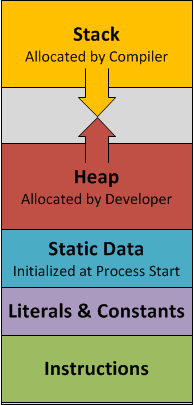
\includegraphics[height=.5\textheight]{images/process-memory-layout}
    \end{column}
  \end{columns}

\end{frame}

\begin{frame}<trans:0>[fragile]{Functions and the stack}

  \begin{columns}
    \begin{column}{.5\textwidth}
      \begin{codeblock}
\alert<4>{int isqrt(int n)
\{
  int i} \alert<6>{= 1};
  \alert<7>{while (i * i < n) \{
    ++i;
  \}
  if (i * i > n) \{
    --i;
  \}}
  \alert<8>{return i;}
\alert<4>{\}}

\alert<2>{int main()
\{
  int num};
  \alert<3>{std::cin >{}> num;}
  \alert<2>{int result} \alert<8>{=} \alert<4>{isqrt(}\alert<5>{num}\alert<4>{)};
  std::cout <{}< result <{}< \bslashn;
\alert<2>{\}}\end{codeblock}

    \end{column}

    \begin{column}{.4\textwidth}
      \begin{tikzpicture}[
        mem/.style={
          minimum width=2cm,
          inner sep=0pt,
          outer sep=0pt,
          draw=black
        },
        frame/.style={
          minimum width=2cm,
          inner sep=0pt,
          outer sep=0pt,
          draw=black,
          thick,
          fill=green!50!white
        },
        var/.style={
          node font=\ttfamily\scriptsize,
          minimum height=.5cm,
          minimum width=2cm,
          draw=black,
          fill=green!30!white,
          inner sep=0pt,
          outer sep=0pt
        },
        anchor=south west]
        \visible<1->{
          \node at (0,0) [
          mem,
          minimum height=7cm,
          label={90:Stack}] {};
        }
        \visible<2-9>{
          \node (main) at (0,4) [
            frame,
            minimum height=2cm,
            label={[yshift=.9cm]0:\scriptsize\tt main}
          ] {};
          \node (result) [
            var,
            above=3ex of main.south,
            label={180:\scriptsize\tt result}
          ] {\only<8->{2}};
          \node (num) [
            var,
            above=0pt of result,
            label={180:\scriptsize\tt num}
          ] {\only<3->{5}};
        }
        \visible<4-8>{
          \node (isqrt) [
            frame,
            below=0pt of main,
            minimum height=2cm,
            label={[yshift=.9cm]0:\scriptsize\tt isqrt}
          ] {};
          \node (i) [
            var,
            above=3ex of isqrt.south,
            label={180:\scriptsize\tt i}
          ] {\only<6>{1}\only<7->{2}};
          \node (n) [
            var,
            above=0pt of i,
            label={180:\scriptsize\tt n}
          ] {\only<5->{5}};
        }
        \visible<2-3,9>{
          \node (main rsp) at ([xshift=-2cm]main.south west) {\scriptsize\tt \%rsp};
          \draw[->] (main rsp) -- +(1.5cm,0);
        }
        \visible<4-8>{
          \node (isqrt rsp) at ([xshift=-2cm]isqrt.south west) {\scriptsize\tt \%rsp};
          \draw[->] (isqrt rsp) -- +(1.5cm,0);
        }
      \end{tikzpicture}
    \end{column}

  \end{columns}

  \uncover<10>{}

\end{frame}

\begin{frame}<0|trans:1>[fragile]{Functions and the stack}

  \begin{columns}
    \begin{column}{.5\textwidth}
      \begin{codeblock}
int isqrt(int n)
\{
  int i\{1\};
  while (i * i < n) \{
    ++i;
  \}
  if (i * i > n) \{
    --i;
  \}
  return i;
\}

int main()
\{
  int num;
  std::cin >{}> num;
  int result\{isqrt(num)\};
  std::cout <{}< result <{}< \bslashn;
\}\end{codeblock}

    \end{column}

    \begin{column}{.4\textwidth}
      \begin{tikzpicture}[
        mem/.style={
          minimum width=2cm,
          inner sep=0pt,
          outer sep=0pt,
          draw=black
        },
        frame/.style={
          minimum width=2cm,
          inner sep=0pt,
          outer sep=0pt,
          draw=black,
          thick,
          fill=green!50!white
        },
        var/.style={
          node font=\ttfamily\scriptsize,
          minimum height=.5cm,
          minimum width=2cm,
          draw=black,
          fill=green!30!white,
          inner sep=0pt,
          outer sep=0pt
        },
        anchor=south west]
        \node (stack) at (0,0) [
          mem,
          minimum height=6cm,
          label={90:Stack}
        ] {};
        \node (main) at (0,3) [
          frame,
          minimum height=2cm,
          label={[yshift=.9cm]0:\scriptsize\tt main}
        ] {};
        \node (result) [
          var,
          above=3ex of main.south,
          label={180:\scriptsize\tt result}
        ] {?};
        \node (num) [
          var,
          above=0pt of result,
          label={180:\scriptsize\tt num}
        ] {5};
        \node (isqrt) [
          frame,
          below=0pt of main,
          minimum height=2cm,
          label={[yshift=.9cm]0:\scriptsize\tt isqrt}
        ] {};
        \node (i) [
          var,
          above=3ex of isqrt.south,
          label={180:\scriptsize\tt i}
        ] {2};
        \node (n) [
          var,
          above=0pt of i,
          label={180:\scriptsize\tt n}
        ] {5};
        \node (isqrt rsp) at ([xshift=-2cm]isqrt.south west) {\scriptsize\tt \%rsp};
        \draw[->] (isqrt rsp) -- +(1.5cm,0);
        \node (description) [below=.1em of stack,align=left] {{\scriptsize The state of the stack just}\\{\scriptsize before returning from isqrt}};
      \end{tikzpicture}
    \end{column}

  \end{columns}

  \uncover<10>{}

\end{frame}

\begin{frame}{Pass by-value, return by-value}

  Given a function

  % \tikzref doesn't work inside \code nor inside \texttt; to be investigated

  \begin{equation*}
    \code{R F(T$_1$ p}\tikzref{p1}\code{$_1$, \ddd, T$_n$ p}\tikzref{pn}\code{$_n$) \{ \ddd{} return E}\tikzref{er}\code{$_R$; \} }
  \end{equation*}

  and a function call

  \begin{equation*}
    \code{R r}\tikzref{r}\code{ = F(E}\tikzref{e1}\code{$_1$, \ddd, E}\tikzref{en}\code{$_n$);}
  \end{equation*}

  \begin{itemize}
  \item<2-> Each \code{p$_i$} is initialized with the value of expression
    \code{E$_i$}
    \begin{itemize}
    \item Every time the function is called a new \code{p$_i$} is created, which
      gets destroyed at the end of the function
    \item NB if \code{E$_i$} is just a variable, \code{p$_i$} is another object
      (a copy) and changing it inside the function doesn't change the original
      object corresponding to the variable
    \end{itemize}
  \item<3-> \code{r} is initialized with the value of expression \code{E$_R$}
  \end{itemize}

  \visible<2->{
    \tikz[remember picture, overlay] \draw[-Stealth,blue,line width=1pt] ([yshift=1ex] e1) -- ([yshift=-1ex]p1);
    \tikz[remember picture, overlay] \draw[-Stealth,blue,line width=1pt] ([yshift=1ex] en) -- ([yshift=-1ex]pn);
  }
  \visible<3->{
    \tikz[remember picture, overlay] \draw[-Stealth,brown,line width=1pt] ([yshift=-1ex] er) -- ([yshift=1ex]r);
  }

\end{frame}

\begin{frame}{Stack frame}

  \begin{itemize}[<+->]
  \item A piece of memory allocated and dedicated to the execution of a function
  \item It contains local variables (including function parameters), return
    address, saved registers, \ldots
  \item Managed in a Last-In, First-Out (LIFO) way
  \item The size of the stack frame is computed by the compiler
  \item There is a special register (the stack pointer register, \code{\%rsp})
    that indicates the frame of the currently running function
  \item At runtime the allocation/deallocation of a frame consists simply in
    subtracting/adding that frame size to the stack pointer register
  \end{itemize}
\end{frame}

\begin{frame}[fragile]{Conditional/ternary operator expression}

  \begin{center}
    \textit{expression}$_{condition}$ \code{?} \textit{expression}$_{true}$ \code{:} \textit{expression}$_{false}$
  \end{center}

  \begin{codeblock}
int gcd(int a, int b)
\{
  return (b == 0) \alert{?} a \alert{:} gcd(b, a \% b);
\}\end{codeblock}

  \begin{itemize}
  \item Evaluate \textit{expression}$_{condition}$, whose value is of type
    (convertible to) \code{bool}
  \item If \code{true}, \textit{expression}$_{true}$ is evaluated and the
    resulting value is the value of the whole expression
  \item If \code{false}, \textit{expression}$_{false}$ is evaluated and the
    resulting value is the value of the whole expression
  \end{itemize}

  \begin{itemize}
  \item Similar to an \code{if} statement, but usable (and useful) where only an
    expression is allowed
  \item The types of \textit{expression}$_{true}$ and
    \textit{expression}$_{false}$ are subject to some constraints, but let's
    assume that they have to be the same
  \end{itemize}

\end{frame}

\begin{frame}[fragile]{\code{break} and \code{continue} for loops}

  \begin{itemize}
  \item<1-> Within a loop block, the \code{break} statement allows to terminate
    the loop
  \item<2-> Within a loop block, the \code{continue} statement allows to jump to
    the end of the current iteration of the loop
  \item<3> The same effect can be obtained with appropriate use of conditionals,
    but the resulting code may be more complicated (\href{https://isocpp.github.io/CppCoreGuidelines/CppCoreGuidelines#es77-minimize-the-use-of-break-and-continue-in-loops}{ES.77})
  \end{itemize}
\end{frame}

\begin{frame}[fragile]{Object initialization with braces}

  \begin{itemize}
  \item An object can be initialized specifying its value between \code{\{\}}

    \begin{codeblock}
int i\{123\};
float f\{123.F\};
std::string s\{"hello"\};\end{codeblock}

  \item Introduced as a \textit{universal} form of initialization that could
    replace all others, but there are situations where it's not usable

  \item Protects against \textit{narrowing}, i.e. loss of information caused by
    implicit conversions

    % try with clang, gcc is too forgiving and gives warnings
    % see `-Wno-narrowing` at https://gcc.gnu.org/onlinedocs/gcc-9.1.0/gcc/C_002b_002b-Dialect-Options.html
    \begin{codeblock}
double d\{1.\};         // ok, no conversion
float f1\{1.\};         // ok, no information loss
float f2\{d\};          // error
float f3\{9\textquotesingle{}999\textquotesingle{}999\};  // ok, no information loss
float f4\{99\textquotesingle{}999\textquotesingle{}999\}; // error
int i\{1.\};            // error
int g\{d\};             // error\end{codeblock}

  \item To force narrowing, use \code{static_cast} or initialize with \code{=} or
    \code{()}
  \end{itemize}
\end{frame}

\begin{frame}[fragile]{\code{char}}

  Type representing a character

  \begin{itemize}[<+->]
  \item Set of values: letters in the alphabet (lower- and upper-case), digits,
    punctuation marks, some special characters, \ldots
  \item Size: typically 1 byte, but not necessarily
  \item Representation: let's assume the
    \href{https://en.wikipedia.org/wiki/ASCII}{ASCII} encoding
  \item Literals: characters between single quotes
    \begin{itemize}[<.->]
    \item \code{\upquote{a} \upquote{B} \upquote{7} \upquote{,} \upquote{?} \upquote{\#} \upquote{/}}
    \end{itemize}
  \item Some character literals need to be expressed as \code{\bslash}-escaped
    sequences
    \begin{itemize}[<.->]
    \item \code{\upquote{\bslash\textquotesingle} \upquote{\bslash\bslash} \upquote{\bslash{n}} \upquote{\bslash{t}} \upquote{\bslash{0}}}
    \end{itemize}
  \item A \code{char} is an integral type so it supports integral operations
    \begin{itemize}
    \item \code{std::cout <{}< \upquote{9} - \upquote{0}; // 9}
    \item \code{c < \upquote{z};}
    \end{itemize}
  \end{itemize}

\end{frame}

\begin{frame}{Exercises}

  \begin{itemize}
  \item Write a function that takes a \code{char} and returns the corresponding
    lowercase character if it is a letter; the same char otherwise
    \begin{itemize}
    \item e.g. \upquote{A} $\rightarrow$ \upquote{a}, \upquote{a} $\rightarrow$
      \upquote{a}, \upquote{;} $\rightarrow$ \upquote{;}
    \end{itemize}
  \item Write a function that takes two numeric operands of type \code{double}
    and one operator of type \code{char} and returns the result of applying that
    operator to the two operands. For example if the two operands have values
    $2.0$ and $3.0$ respectively and the operator has value \code{\upquote{+}},
    then the function returns a result with value $5.0$. If the operator is
    invalid, the function returns $0$.
  \end{itemize}
\end{frame}
